\documentclass[twoside,onecolumn,11pt,a4paper]{scrartcl}
\usepackage{anuthesis}

\usepackage{fancyhdr}
\usepackage{graphicx}

  \renewcommand{\bottomfraction}{0.7}  

\begin{document}

\pagenumbering{roman}  % first use Roman numerals for page numbers

\begin{titlepage}
\title{\textbf{A Simple Example of a Latex Thesis}\\[2cm]}
 \author{\textbf{Mickey M. Mouse}\\[6cm]
 \textbf{A thesis submitted for the degree of}\\
 \textbf{Bachelor of Science with Honours in Physics of} \\
 \textbf{The Australian National University}\\[1cm]}
 \date{\textbf{October, 2004}}
\maketitle
 \end{titlepage}
 
 \sloppy
 
\chapter*{Declaration}
\addcontentsline{toc}{chapter}{Declaration}

This thesis is an account of research undertaken between February 2004 and 
October 2004 at The Department of Physics, Faculty of Science, 
The Australian National University, Canberra, Australia.

Except where acknowledged in the customary manner, the material 
presented in this thesis is, to the best of my knowledge, original and 
has not been submitted in whole or part for a degree in any 
university.

\vspace{20mm}  % vertical space

\hspace{80mm}\rule{40mm}{.15mm}\par   % horizontal space, line, start new line
\hspace{80mm} Mickey M. Mouse\par
\hspace{80mm} October, 2004

% include statements effectively insert the contents of the named file.
% They are not necessary, but are useful for organising your work.
% They always start a  new page.

\chapter*{Acknowledgements}
\addcontentsline{toc}{chapter}{Acknowledgements}

I would like to thank my lucky stars, and the cat, for not eating me.
  % include the contents of the file thanks.tex

\chapter*{Abstract}
\addcontentsline{toc}{chapter}{Abstract}
\vspace{-1em}
The constraint satisfaction problems (CSPs) are created to model two puzzle games IQ Twist and Zig Zag Puzzler. Both of them have "start", "junior", "expert", "master" and "wizard" difficulties. With regard to CSPs for both games, the variables, domains, and constraints are mainly discussed. Meanwhile, in the process of discussing constraints, the 2D rotation matrix is introduced to clarify the pieces' configurations for the 2D game (IQ Twist), and the 3D rotation matrix is introduced to clarify the pieces' configurations for the 3D game (Zig Zag Puzzler). After that, these models are encoded by Minizinc which is a constraint modeling language. Through Minizinc IDE, the Minizinc is transferred to Flatzinc, a solver input language that is understood by a wide range of solvers. Therefore, nine solvers are used to execute these problems by different interfaces, which create the bridges between each solver and the Flatzinc file. For IQ Twist, the solvers' performances are not strongly related to the difficulties, while there is an obvious negative correlation between the performance and difficulties in Zig Zag Puzzler. Finally, there are three solvers Chuffed, OR-Tools and PicatSAT, which perform the 100 percent coverage. In other words,  they solve each problem in thirty minutes. More specifically, Chuffed achieve the optimal performance in most problems because it solves each problem in 20 seconds, while the other two need more time.
\\
\\
\\
\\\textbf{Keywords:} CSPs, IQ Twist, Zig Zag Puzzler, rotation matrix, Minizinc, Flatzinc, Chuffed, OR-Tools, PicatSAT.


  % include the file abstract.tex

\tableofcontents
\listoffigures % makes a list of figures
%\listoftables  % uncomment this if you have tables

\pagenumbering{arabic} % switch to Arabic numerals for page numbers
\setcounter{page}{1}  % set page number to 1

\pagenumbering{arabic} % switch to Arabic numerals for page numbers
\setcounter{page}{1}  % set page number to 1

\chapter{Figures and References}

This chapter gives examples of how to reference the literature, and how to include a figure. To use Latex effectively you either need someone you can ask questions of, or a good book. The book I find most useful is Math into Latex.

Here's an example of including a figure. Figures need to have size information in them. The only ones I know how to make work are encapsulated postscript files, or eps files. If your figures are not in eps form you may need to find a graphics program which can convert formats.
% The percent symbol indicates a comment which is not read by Latex. 
%They are useful because a blank line, means a new paragraph.
\begin{figure}
  \begin{center}  % center environment centers the graphic on the page
    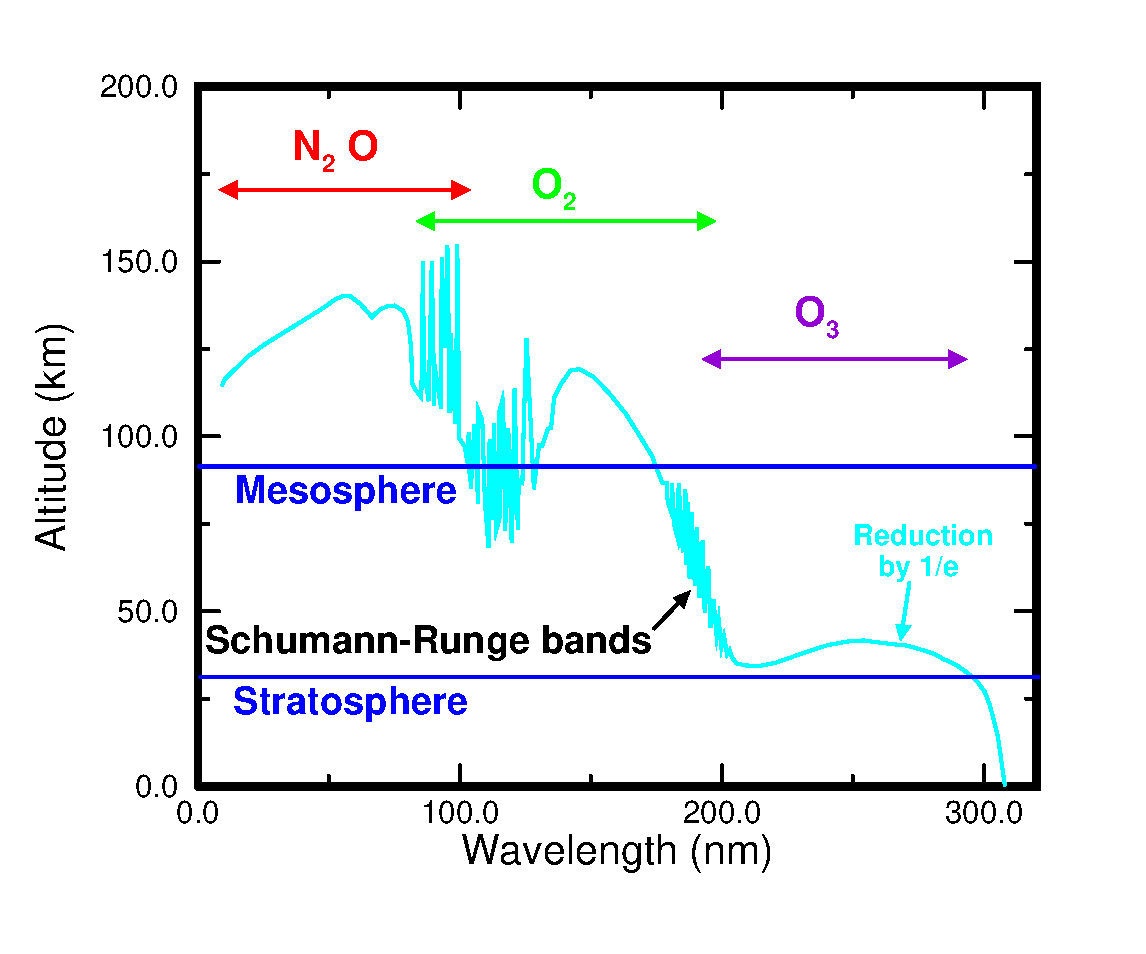
\includegraphics[width=10cm]{fig1.eps}
  \end{center}
\caption{This is an example of how to include an eps (encapsulated postscript) figure. Maths is OK in the caption $\epsilon^2 =\Delta$. }
\label{fig:Label}
\end{figure}
%
Notice how I can refer to the figure, Fig.~\ref{fig:Label}. 

And this sentence includes an example citation \cite{Biundo2016CompanionSurvey}. Although I, Pascal, think that the bibliographystyle still needs some fine-tuning. And we need to check if and how authors can be cited by name. (Only loosely related: some useful packages should be included as well, such as hyperref to get links.)
  % include the file chapter1.tex

\chapter{How to do Maths}

This chapter gives some examples of including maths into your thesis.

An example of a differential equation:
%
\begin{equation} 
\frac{\partial^2 \psi}{\partial t^2} -2i \frac{m v_\theta}{r} \frac{\partial \psi}{\partial t} -
\frac{1}{r} \frac{\partial}{\partial r} \left( r c^{2} \frac{\partial \psi}{\partial r} \right) 
+ \frac{m^{2}}{r^2} \left( c^{2} - v_\theta^{2} \right)  \psi  
= 0 \; .
\label{wave equation}
\end{equation}
%
Equations can also be inline $\phi (t, r, \theta, z) = \psi(t,r) e^{-i m \theta}$, i.e. not displayed separately from the text. I can also refer to equations, Eq.~(\ref{wave equation}).
 % include the file chapter2.tex

\bibliographystyle{alpha}
\bibliography{MyBibliography}  % include the file MyBibliography.tex

\end{document}
